\documentclass[10pt,a4paper]{article}
\usepackage[margin=2cm]{geometry}
\usepackage[T1]{fontenc}
\usepackage{lmodern}
\usepackage{amsmath,amssymb,booktabs,multirow,colortbl}
\usepackage[table]{xcolor}
\usepackage{pgfplots}
\pgfplotsset{compat=1.18}
\usepackage{float}
\usepackage[hidelinks]{hyperref}
\usepackage{titlesec,enumitem}
\titleformat{\section}{\large\bfseries}{\thesection}{0.6em}{}
\titleformat{\subsection}{\normalsize\bfseries}{\thesubsection}{0.5em}{}
\setlist{itemsep=1pt,topsep=3pt}

\definecolor{cmag}{HTML}{1F6F8B}
\definecolor{cfis}{HTML}{6A8F3A}
\definecolor{cgrad}{HTML}{C0612B}
\definecolor{ctier}{HTML}{7B3F98}
\definecolor{crand}{HTML}{8A939C}
\newcommand{\gain}[1]{\textcolor{cmag}{\textbf{#1}}}
\pgfplotsset{
  accplot/.style={width=0.49\textwidth,height=5.6cm,grid=major,grid style={gray!20},
    tick label style={font=\scriptsize},label style={font=\footnotesize},title style={font=\small\bfseries},
    legend style={font=\scriptsize,draw=none,fill=white,fill opacity=0.85,text opacity=1},
    legend cell align=left,mark size=1.3pt},
  pslc/.style={black,densely dotted,thick,mark=square*,mark options={solid}},
  pslcmap/.style={black,thick,mark=square*},
  pgrad/.style={cgrad,thick,mark=*},
  pmag/.style={cmag,very thick,mark=*},
  pfis/.style={cfis,thick,dashed,mark=diamond*,mark options={solid}},
  phyb/.style={crand,thick,mark=o},
  pmap/.style={cmag,very thick,mark=*},
  pjoint/.style={cfis,thick,dashed,mark=diamond*,mark options={solid}},
  pnf/.style={cgrad,thick,mark=triangle*},
  ptier/.style={ctier,very thick,mark=*}}

\setlength{\emergencystretch}{2em}
\begin{document}

\begin{center}
{\LARGE\bfseries Contribution Results}\\[4pt]
{\large Reliable Hybrid SLC/MLC ReRAM Crossbars for Transformers}\\[4pt]
Shivansh Mittal, Sarvesh Joshi, Thumati Naveen Chandra Chowdary, Aryan Chakravorty\\
CS5290 Memory-Centric Computer Architecture, Indian Institute of Technology Guwahati
\end{center}

\section*{Overview}
The baseline is the HyFlexPIM hybrid (SVD components ranked by the loss gradient, 20\% in SLC), with all-SLC and
all-MLC chips as references (see \emph{Baseline Results}). We contribute five things, in the order of the
report: (1) a verified cell-level crossbar model and the finding that stuck cells are the limiting effect;
(2) a Fisher-information estimate of each component's damage, which shows that ranking by singular value
(magnitude) is close to the best placement; (3) fault-aware mapping; (4) tier-aware training; (5) evidence
that (2) and (3) hold on MNLI. Every method is tested on the same simulated chips as the baseline, so
differences within an experiment are paired (mean $\pm$ standard error, in accuracy points unless stated). The
hybrid chip uses 9.2 cells per weight, 34\% fewer than all-SLC.

\section{Contribution 1: cell-level crossbar model and characterisation}
\textbf{What.} A simulator that stores every weight as a real crossbar would: 8-bit integers with one scale
per output column, a differential cell pair for the sign, and 7 SLC or 4 MLC bit slices per sign. Errors are
applied to every cell: programming noise, read noise, level-dependent MLC noise, stuck cells in three spatial
patterns, IR drop, and a fixed ADC with bit-serial inputs. Self-tests show that, with all errors off, it
equals exact 8-bit integer arithmetic (relative error $<10^{-4}$), and an error-free chip stays within about one
point of the digital model. HyFlexPIM instead perturbs whole weights, $\tilde W=W\odot(1+\eta)$, at a single
noise level, so these effects cannot be studied there.

\begin{table}[H]
\centering\small
\caption{Our placements under each non-ideality, one at a time, with 20\% SLC: accuracy (\%) of magnitude and
Fisher, and the difference of magnitude to the HyFlexPIM gradient hybrid and to all-SLC on the same chips
(baseline values in the \emph{Baseline Results}; complete sweeps in Appendix A.4).}\label{t:chip}
\resizebox{\textwidth}{!}{%
\begin{tabular}{@{}l cccc c cccc@{}}
\toprule
& \multicolumn{4}{c}{BERT-Base} && \multicolumn{4}{c}{DistilBERT} \\
\cmidrule{2-5}\cmidrule{7-10}
Condition & Magnitude & Fisher & vs HyFlexPIM & vs all-SLC && Magnitude & Fisher & vs HyFlexPIM & vs all-SLC \\
\midrule
No errors & 90.6 & 89.6 & +0.3 & +0.9 && 88.8 & 89.1 & +0.1 & +0.2 \\
\midrule
Read noise $\sigma_r=2\%$ & 90.1 & 89.7 & +0.3 & +1.1 && 88.4 & 88.2 & +0.3 & +0.1 \\
Read noise $\sigma_r=5\%$ & 82.5 & 82.7 & +5.8 & +2.5 && 83.3 & 83.2 & +2.9 & -1.2 \\
$\sigma=5\%$, middle MLC levels $\times2$ & 88.4 & 88.4 & +0.5 & +0.2 && 88.0 & 87.9 & +1.0 & -0.4 \\
ADC 6 bits (bit-serial) & 90.0 & 90.5 & +0.5 & +0.7 && 89.7 & 88.8 & +1.3 & +1.7 \\
ADC 5 bits (bit-serial) & 51.1 & 51.6 & -1.8 & +0.0 && 70.6 & 70.9 & -6.7 & -0.3 \\
IR drop $r=3\times10^{-4}$ & 90.4 & 91.1 & -0.1 & +1.5 && 89.7 & 89.3 & +0.1 & +0.2 \\
IR drop $r=3\times10^{-3}$ & 76.8 & 72.8 & +0.5 & +18.3 && 73.4 & 72.6 & -1.3 & +3.3 \\
\midrule
1\% stuck cells, scattered & 56.4 & 55.6 & +3.8 & -5.0 && 62.5 & 60.0 & +7.5 & -11.7 \\
1\% stuck cells, $3\times3$ clusters & 54.0 & 53.1 & +2.5 & -12.7 && 56.1 & 57.3 & -0.3 & -24.1 \\
1\% stuck cells, bit lines & 50.4 & 52.2 & -0.6 & -6.6 && 54.7 & 56.3 & +2.5 & -16.5 \\
\bottomrule
\end{tabular}}
\end{table}

\noindent\textbf{Takeaways.}
\begin{itemize}
\item Under read noise, level-dependent noise, a 6-bit ADC and moderate IR drop, the magnitude and Fisher
hybrids stay within about a point of all-SLC or above it, and magnitude is 2.9--5.8 points ahead of the
HyFlexPIM hybrid at 5\% read noise. A 6-bit ADC suffices for the hybrid.
\item \textbf{Stuck cells are the limiting effect}: at 1\% stuck cells every hybrid placement loses 26--40 points
against its error-free accuracy, for every fault pattern, and even all-SLC loses 8--33. Contributions 3 and 4
address this.
\end{itemize}

\section{Contribution 2: Fisher damage estimate and magnitude placement}
\textbf{What.} The expected rise in loss if component $r$ is stored in MLC, summed over every number it stores
(its column $\sigma_r v_r$ in the first crossbar and its row $u_r$ in the second):
\[
D_r=s_r^2\sum_j F(\sigma_r v_{rj})+\sum_i t_i^2F(u_{ir}),
\]
where $F$ is the empirical Fisher information (loss sensitivity) of each stored number and $s_r$, $t_i$ are the
8-bit column scales that turn a fixed cell noise into a weight error. $D_r$ is the principled estimate of what
placement should minimise. We compare it with the HyFlexPIM gradient and with plain magnitude $|\sigma_r|$.

\begin{figure}[H]
\centering
\begin{tikzpicture}
\begin{axis}[accplot,title={BERT-Base},xlabel={Programming noise $\sigma$ (\% of $G_{\max}$)},ylabel={Accuracy (\%)},
  xtick={0,1,2,3,5,7.5,10},ymin=60,ymax=92,legend pos=south west]
\addplot[pslc] table[x=x,y=all_slc]{data/noise_bert.dat}; \addlegendentry{All SLC}
\addplot[pmag] table[x=x,y=magnitude]{data/noise_bert.dat}; \addlegendentry{Magnitude}
\addplot[pfis] table[x=x,y=fisher]{data/noise_bert.dat}; \addlegendentry{Fisher}
\addplot[pgrad] table[x=x,y=gradient]{data/noise_bert.dat}; \addlegendentry{HyFlexPIM gradient}
\end{axis}
\end{tikzpicture}\hfill
\begin{tikzpicture}
\begin{axis}[accplot,title={DistilBERT},xlabel={Programming noise $\sigma$ (\% of $G_{\max}$)},
  xtick={0,1,2,3,5,7.5,10},ymin=60,ymax=92]
\addplot[pslc] table[x=x,y=all_slc]{data/noise_distil.dat};
\addplot[pmag] table[x=x,y=magnitude]{data/noise_distil.dat};
\addplot[pfis] table[x=x,y=fisher]{data/noise_distil.dat};
\addplot[pgrad] table[x=x,y=gradient]{data/noise_distil.dat};
\end{axis}
\end{tikzpicture}
\caption{Accuracy against programming noise, 20\% SLC, mean of 5 chips.}
\end{figure}

\begin{figure}[H]
\centering
\begin{tikzpicture}
\begin{axis}[accplot,title={BERT-Base, $\sigma=7.5\%$},xlabel={Share of components in SLC (\%)},ylabel={Accuracy (\%)},
  xtick={0,10,20,30,50,100},ymin=50,ymax=90,legend pos=south east]
\addplot[pmag] table[x=x,y=magnitude]{data/share_bert_075.dat}; \addlegendentry{Magnitude}
\addplot[pfis] table[x=x,y=fisher]{data/share_bert_075.dat}; \addlegendentry{Fisher}
\addplot[pgrad] table[x=x,y=gradient]{data/share_bert_075.dat}; \addlegendentry{HyFlexPIM gradient}
\end{axis}
\end{tikzpicture}\hfill
\begin{tikzpicture}
\begin{axis}[accplot,title={DistilBERT, $\sigma=7.5\%$},xlabel={Share of components in SLC (\%)},
  xtick={0,10,20,30,50,100},ymin=50,ymax=90]
\addplot[pmag] table[x=x,y=magnitude]{data/share_distil_075.dat};
\addplot[pfis] table[x=x,y=fisher]{data/share_distil_075.dat};
\addplot[pgrad] table[x=x,y=gradient]{data/share_distil_075.dat};
\end{axis}
\end{tikzpicture}
\caption{Accuracy against the share of components in SLC at $\sigma=7.5\%$, mean of 20 chips; 0\% is all-MLC,
100\% all-SLC.}
\end{figure}

\begin{table}[H]
\centering\small
\caption{Paired difference to magnitude, in correctly classified sentences out of 872 (mean $\pm$ standard
error; 100 chips per noise level, 300 overall, all SLC shares).}\label{t:paired}
\begin{tabular}{@{}llrrrr@{}}
\toprule
Model & Placement & $\sigma=3\%$ & 5\% & 7.5\% & All \\
\midrule
\multirow{2}{*}{BERT-Base} & Fisher & $-0.1\pm0.5$ & $-0.1\pm0.7$ & $+1.4\pm1.9$ & $+0.4\pm0.7$ \\
 & HyFlexPIM gradient & $-1.2\pm0.7$ & $-10.4\pm1.6$ & $-40.4\pm5.0$ & $-17.3\pm2.0$ \\
\midrule
\multirow{2}{*}{DistilBERT} & Fisher & $-0.4\pm0.7$ & $-1.3\pm0.7$ & $+0.0\pm1.7$ & $-0.6\pm0.7$ \\
 & HyFlexPIM gradient & $-0.9\pm0.7$ & $-4.0\pm1.0$ & $-18.4\pm2.6$ & $-7.8\pm1.1$ \\
\bottomrule
\end{tabular}
\end{table}

\begin{table}[H]
\centering\small
\caption{Smallest SLC share within half a point of all-SLC (shares tested: 5, 10, 20, 30, 50\%), and the
resulting cells per weight relative to all-SLC.}\label{t:need}
\begin{tabular}{@{}llccc@{}}
\toprule
Model & Placement & $\sigma=3\%$ & $\sigma=5\%$ & $\sigma=7.5\%$ \\
\midrule
\multirow{2}{*}{BERT-Base} & Magnitude & \gain{5\%} (59\% of cells) & \gain{5\%} (59\%) & \gain{30\%} (70\%) \\
 & HyFlexPIM gradient & 5\% (59\%) & 10\% (61\%) & not reached at 50\% \\
\midrule
\multirow{2}{*}{DistilBERT} & Magnitude & 5\% (59\%) & \gain{10\%} (61\%) & \gain{50\%} (79\%) \\
 & HyFlexPIM gradient & 5\% (59\%) & 20\% (66\%) & not reached at 50\% \\
\bottomrule
\end{tabular}
\end{table}

\noindent\textbf{Takeaways.}
\begin{itemize}
\item \textbf{Fisher and magnitude choose the same components}: rank correlation 0.96--0.97 on MNLI, and a paired
difference within about one sentence in 872 at every noise level on SST-2 (Table~\ref{t:paired}).
\item \textbf{Both beat the HyFlexPIM gradient at high noise}: by $+2.8\pm0.8$ and $+2.2\pm0.3$ points at 20\% SLC and
$\sigma=7.5\%$, and by $+11.9\pm1.7$ points on BERT-Base at 5\% SLC.
\item \textbf{Why}: the column of component $r$ holds $\sigma_r v_r$, so its scale, and the weight error a cell
noise causes, is proportional to $|\sigma_r|$. Fisher multiplies this error size by the sensitivity; that it
agrees with magnitude suggests the error size dominates. The gradient ignores the error size.
\item \textbf{Practical result}: magnitude needs no data or gradients and half the SLC share of the gradient at
$\sigma=5\%$ (Table~\ref{t:need}).
\end{itemize}

\section{Contribution 3: fault-aware mapping}
\textbf{What.} The components of an SVD layer can be stored in any order. After a chip is tested, each
component is placed in the slot whose stuck cells hurt it least: the cost of component $r$ in slot $s$ is the
Fisher-weighted squared error that slot's stuck cells would cause, and the Hungarian algorithm finds the best
assignment. It needs no extra hardware or retraining. Joint mapping, which also chooses the tier per chip, is
tested as an extension.

\begin{figure}[H]
\centering
\begin{tikzpicture}
\begin{axis}[accplot,title={BERT-Base},xlabel={Stuck cells $p$ (\% of cells)},ylabel={Accuracy (\%)},
  symbolic x coords={0.2,0.5,1,2},xtick=data,ymin=45,ymax=93,legend pos=south west]
\addplot[pslc] table[x=x,y=slc]{data/recover_bert.dat}; \addlegendentry{All SLC}
\addplot[pslcmap] table[x=x,y=slc_map]{data/recover_bert.dat}; \addlegendentry{All SLC + mapping}
\addplot[phyb] table[x=x,y=hyb]{data/recover_bert.dat}; \addlegendentry{Hybrid, no mitigation}
\addplot[pmap] table[x=x,y=hyb_map]{data/recover_bert.dat}; \addlegendentry{Hybrid + fault-aware mapping}
\addplot[pjoint] table[x=x,y=joint]{data/recover_bert.dat}; \addlegendentry{Hybrid + joint mapping}
\end{axis}
\end{tikzpicture}\hfill
\begin{tikzpicture}
\begin{axis}[accplot,title={DistilBERT},xlabel={Stuck cells $p$ (\% of cells)},
  symbolic x coords={0.2,0.5,1,2},xtick=data,ymin=45,ymax=93]
\addplot[pslc] table[x=x,y=slc]{data/recover_distil.dat};
\addplot[pslcmap] table[x=x,y=slc_map]{data/recover_distil.dat};
\addplot[phyb] table[x=x,y=hyb]{data/recover_distil.dat};
\addplot[pmap] table[x=x,y=hyb_map]{data/recover_distil.dat};
\addplot[pjoint] table[x=x,y=joint]{data/recover_distil.dat};
\end{axis}
\end{tikzpicture}
\caption{Accuracy against the share of stuck cells, no programming noise, mean of 10 chips. The hybrid uses
magnitude placement with 20\% SLC.}\label{f:map}
\end{figure}

\begin{table}[H]
\centering\small
\caption{Paired gain of fault-aware mapping over no mitigation (hybrid, magnitude, 20\% SLC), and of joint
tier-and-slot mapping over fault-aware mapping, in accuracy points (mean $\pm$ s.e. over 10 chips).}\label{t:mapgain}
\setlength{\tabcolsep}{3.5pt}
\resizebox{\textwidth}{!}{%
\begin{tabular}{@{}ll cccc ccc cc@{}}
\toprule
& & \multicolumn{4}{c}{Stuck cells, no noise} & \multicolumn{3}{c}{Stuck cells, $\sigma=5\%$} & \multicolumn{2}{c}{1\% stuck} \\
\cmidrule(lr){3-6}\cmidrule(lr){7-9}\cmidrule(l){10-11}
& Model & 0.2\% & 0.5\% & 1\% & 2\% & 0.2\% & 0.5\% & 1\% & clusters & lines \\
\midrule
\multirow{2}{*}{Mapping gain} & BERT & $+1.6\pm0.3$ & $+8.9\pm2.0$ & $+9.2\pm2.6$ & $+2.1\pm1.2$ & $+2.5\pm0.6$ & $+10.2\pm2.1$ & $+6.0\pm1.7$ & $+10.6\pm2.3$ & $+6.8\pm2.2$ \\
 & Distil & $+1.3\pm0.5$ & $+7.2\pm3.3$ & $+4.6\pm3.4$ & $+3.1\pm1.1$ & $+2.3\pm0.5$ & $+8.1\pm1.2$ & $+5.6\pm3.5$ & $+12.6\pm2.1$ & $+13.9\pm3.3$ \\
\midrule
\multirow{2}{*}{Joint $-$ mapping} & BERT & $-0.1\pm0.2$ & $-1.3\pm0.8$ & $+3.2\pm2.2$ & $-2.8\pm0.9$ & $-0.3\pm0.3$ & $-2.5\pm1.9$ & $+3.6\pm2.0$ & $-2.8\pm2.7$ & $-0.1\pm1.9$ \\
 & Distil & $-0.1\pm0.1$ & $+0.2\pm0.7$ & $+0.7\pm2.0$ & $+1.4\pm1.6$ & $-0.7\pm0.4$ & $-0.7\pm0.8$ & $-2.0\pm3.1$ & $+7.0\pm2.3$ & $-5.3\pm2.4$ \\
\bottomrule
\end{tabular}}
\end{table}

\noindent\textbf{Takeaways.}
\begin{itemize}
\item \textbf{Mapping helps in every setting}, by 1.3--13.9 points; at 0.5\% stuck cells BERT-Base rises from
76.6\% to 85.6\%, and the spread over chips falls from 6.7 to 1.2 points. Gains are largest for clusters and
broken lines.
\item \textbf{Joint mapping adds nothing reliable}: its second-order cost underrates the large error of a stuck
high-order cell, so the benefit comes from the choice of slot, not of tier.
\item \textbf{Mapping alone falls behind all-SLC from 0.5\% stuck cells}, which contribution 4 closes.
\end{itemize}

\section{Contribution 4: tier-aware training}
\textbf{What.} Fine-tuning for 2 epochs on a freshly simulated chip at every step (5\% noise, 0.5\% stuck cells);
the loss is measured on the damaged weights and the update applied to the clean ones (straight-through).
Tier-aware training simulates the real hybrid layout, so each component trains under the errors of its own
tier; the tier-unaware variants put every component on SLC cells, with noise only or with noise and stuck
cells.

\begin{figure}[H]
\centering
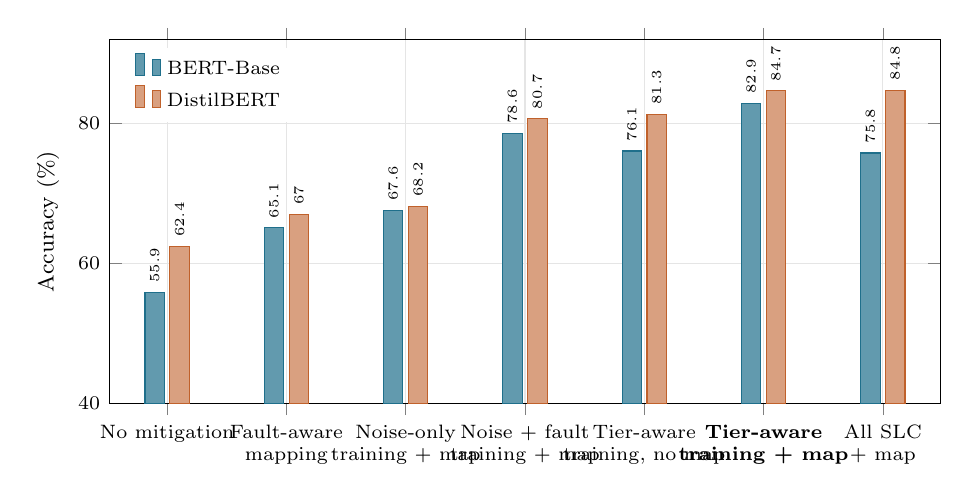
\begin{tikzpicture}
\begin{axis}[ybar,width=\textwidth,height=6.2cm,bar width=7pt,ymin=40,ymax=92,ylabel={Accuracy (\%)},
  symbolic x coords={None,Map,NoiseT,FaultT,TierNoMap,Tier,SLC},xtick=data,
  xticklabels={{No mitigation},{Fault-aware\\mapping},{Noise-only\\training + map},{Noise + fault\\training + map},{Tier-aware\\training, no map},{\textbf{Tier-aware}\\\textbf{training + map}},{All SLC\\+ map}},
  xticklabel style={font=\scriptsize,align=center},tick label style={font=\scriptsize},label style={font=\footnotesize},
  nodes near coords,nodes near coords style={font=\tiny,rotate=90,anchor=west},
  legend style={font=\scriptsize,draw=none,at={(0.02,0.98)},anchor=north west},grid=major,grid style={gray!20},
  enlarge x limits=0.08]
\addplot[fill=cmag!70,draw=cmag] coordinates {(None,55.9) (Map,65.1) (NoiseT,67.6) (FaultT,78.6) (TierNoMap,76.1) (Tier,82.9) (SLC,75.8)};
\addplot[fill=cgrad!60,draw=cgrad] coordinates {(None,62.4) (Map,67.0) (NoiseT,68.2) (FaultT,80.7) (TierNoMap,81.3) (Tier,84.7) (SLC,84.8)};
\legend{BERT-Base,DistilBERT}
\end{axis}
\end{tikzpicture}
\caption{Accuracy at 1\% stuck cells, no programming noise, mean of 10 chips. All bars except the last are the
hybrid chip (magnitude placement, 20\% SLC).}\label{f:bar}
\end{figure}

\begin{table}[H]
\centering\small
\caption{Paired differences of tier-aware training + mapping, in accuracy points (mean $\pm$ s.e., 10 chips).}\label{t:trpaired}
\setlength{\tabcolsep}{3.5pt}
\resizebox{\textwidth}{!}{%
\begin{tabular}{@{}ll cccc ccc cc@{}}
\toprule
& & \multicolumn{4}{c}{Stuck cells, no noise} & \multicolumn{3}{c}{Stuck cells, $\sigma=5\%$} & \multicolumn{2}{c}{1\% stuck} \\
\cmidrule(lr){3-6}\cmidrule(lr){7-9}\cmidrule(l){10-11}
Compared with & Model & 0.2\% & 0.5\% & 1\% & 2\% & 0.2\% & 0.5\% & 1\% & clusters & lines \\
\midrule
\multirow{2}{*}{mapping only} & BERT & $-1.2\pm0.2$ & $+2.7\pm0.5$ & $+17.8\pm2.2$ & $+0.8\pm1.0$ & $+1.6\pm0.5$ & $+7.4\pm0.8$ & $+22.4\pm1.8$ & $+20.7\pm1.6$ & $+20.8\pm2.8$ \\
 & Distil & $-0.1\pm0.2$ & $+3.0\pm0.8$ & $+17.7\pm2.7$ & $+4.1\pm2.4$ & $+0.5\pm0.4$ & $+3.9\pm0.6$ & $+14.7\pm2.4$ & $+14.9\pm2.4$ & $+16.5\pm3.1$ \\
\midrule
\multirow{2}{*}{noise + fault training} & BERT & $-1.0\pm0.2$ & $-0.4\pm0.4$ & $+4.3\pm2.2$ & $+2.2\pm1.0$ & $-0.6\pm0.4$ & $+0.4\pm0.3$ & $+7.5\pm1.8$ & $+6.2\pm1.7$ & $+5.1\pm3.7$ \\
 & Distil & $-0.4\pm0.2$ & $-0.1\pm0.2$ & $+4.0\pm0.6$ & $+2.4\pm1.7$ & $-0.5\pm0.3$ & $+0.5\pm0.3$ & $+2.3\pm1.6$ & $+2.7\pm1.3$ & $+2.8\pm0.8$ \\
\midrule
\multirow{2}{*}{all SLC + mapping} & BERT & $-0.8\pm0.3$ & $+4.6\pm0.7$ & $+7.1\pm3.3$ & $-2.9\pm2.2$ & $+2.9\pm1.4$ & $+5.4\pm1.0$ & $+4.0\pm1.7$ & $+3.7\pm1.4$ & $+0.2\pm3.0$ \\
 & Distil & $+0.3\pm0.2$ & $+0.5\pm0.5$ & $-0.0\pm0.9$ & $-4.9\pm3.1$ & $+0.7\pm0.3$ & $+0.1\pm0.3$ & $-0.9\pm2.4$ & $-2.2\pm1.2$ & $+3.0\pm1.9$ \\
\bottomrule
\end{tabular}}
\end{table}

\begin{table}[H]
\centering\small
\caption{Accuracy (\%) under programming noise alone (no stuck cells), hybrid with 20\% SLC by magnitude,
mean of 10 chips; $\sigma=0$ is an error-free chip.}\label{t:trnoise}
\begin{tabular}{@{}lccc@{\hskip 14pt}ccc@{}}
\toprule
& \multicolumn{3}{c}{BERT-Base} & \multicolumn{3}{c}{DistilBERT} \\
\cmidrule(r){2-4}\cmidrule(l){5-7}
Training & $\sigma=0$ & 5\% & 7.5\% & 0 & 5\% & 7.5\% \\
\midrule
No training & 89.7 & 88.7 & 84.2 & 89.1 & 88.2 & 85.6 \\
Noise-only training & 89.9 & 89.7 & 86.3 & 87.4 & 87.6 & 85.6 \\
Noise + fault training & \textbf{90.9} & \textbf{89.9} & \textbf{88.8} & \textbf{89.9} & \textbf{89.3} & 87.6 \\
Tier-aware training & 89.4 & 89.3 & 88.3 & 87.8 & 88.4 & \textbf{88.0} \\
\bottomrule
\end{tabular}
\end{table}

\noindent\textbf{Takeaways.}
\begin{itemize}
\item \textbf{Stuck cells must be injected}: noise-only training gives no consistent gain under stuck cells.
\item \textbf{Knowing the tiers helps where errors are dense}: tier-aware training beats tier-unaware training at
1\% stuck cells and with noise, and is slightly behind at 0.2\% (cost 0.3 / 1.3 points on an error-free chip).
\item \textbf{Training and mapping are complementary}, and together \textbf{close the gap to all-SLC}: the hybrid
matches or beats all-SLC with mapping up to 1\% scattered stuck cells, with 34\% fewer cells.
\end{itemize}

\section{Contribution 5: generalisation to MNLI}
\begin{table}[H]
\centering\small
\caption{MNLI (three classes, chance 33.3\%): paired results, in accuracy points (mean $\pm$ s.e.). Raw
accuracies are in Appendix A.6.}\label{t:mnli}
\begin{tabular}{@{}lcc@{}}
\toprule
& BERT-Base & DistilBERT \\
\midrule
Fisher $-$ magnitude, $\sigma=5\%$, all SLC shares (100 chips) & $-0.2\pm0.2$ & $-0.2\pm0.1$ \\
HyFlexPIM gradient $-$ magnitude, same chips & $-3.4\pm0.4$ & $-0.5\pm0.2$ \\
Fault-aware mapping gain at 0.5\% stuck cells (10 chips) & $+20.1\pm3.0$ & $+18.8\pm3.2$ \\
\bottomrule
\end{tabular}
\end{table}

\noindent Magnitude again matches Fisher and beats the gradient on BERT-Base, and fault-aware mapping recovers
about 20 points at 0.5\% stuck cells. MNLI also exposed that one 8-bit scale for the vector between a tier's
two crossbars costs up to 11 points even without errors, so only placements with equal tier sizes are compared.

\section{First-order ADC cost estimate}
Savings elsewhere in this document are counted in memory cells. ADCs dominate the power of crossbar
accelerators (58\% of tile power and 31\% of tile area in ISAAC~\cite{isaac}), so we also estimate the ADC
energy of each configuration analytically. We count the conversions of Eq.~(5) of the report: one per output
column, weight slice, 128-row tile and input bit (7 magnitude bits), with the two cells of a differential pair
subtracted before the ADC. Each SVD layer is counted as its two crossbars per tier, so the tiling of the
second crossbar's $k_\tau$ rows is included. The energy per conversion comes from ISAAC's 8-bit SAR ADC at
32\,nm, 1.2\,GS/s, eight ADCs per array group at 16\,mW~\cite{isaac}, i.e.\ 1.67\,pJ per conversion; ISAAC
takes these values from Murmann's ADC survey~\cite{murmann}. ISAAC scales an ADC to other resolutions by
scaling its reference buffer, memory and clock linearly with the number of bits and its capacitive DAC
exponentially~\cite{isaac}. We do not know how the energy splits between these parts, so we report both
bounds: linear ($\propto b$) and exponential ($\propto 2^b$) scaling. The resolution of each configuration is
the smallest that kept it within about a point of the ideal ADC (Section~1): 6 bits for all-SLC and the
hybrid, 7 bits for all-MLC.

\begin{table}[H]
\centering\small
\caption{ADC conversions and ADC energy per token for the encoder linear layers. Energy range: linear to
exponential scaling of the ADC with resolution; the 8-bit all-SLC chip is the reference.}
\begin{tabular}{@{}llcccc@{}}
\toprule
Model & Configuration & ADC bits & Conversions per token & ADC energy per token ($\mu$J) & Relative energy \\
\midrule
\multirow{4}{*}{BERT-Base} & All SLC & 8 & 33.0\,M & 54.9 & 1 \\
 & All SLC & 6 & 33.0\,M & 13.7--41.2 & 0.25--0.75 \\
 & All MLC & 7 & 18.8\,M & 15.7--27.5 & 0.29--0.50 \\
 & Hybrid, 20\% SLC & 6 & 23.0\,M & \phantom{0}9.6--28.8 & 0.17--0.52 \\
\midrule
\multirow{4}{*}{DistilBERT} & All SLC & 8 & 16.5\,M & 27.5 & 1 \\
 & All SLC & 6 & 16.5\,M & \phantom{0}6.9--20.6 & 0.25--0.75 \\
 & All MLC & 7 & \phantom{0}9.4\,M & \phantom{0}7.8--13.7 & 0.29--0.50 \\
 & Hybrid, 20\% SLC & 6 & 11.5\,M & \phantom{0}4.8--14.4 & 0.17--0.52 \\
\bottomrule
\end{tabular}
\end{table}

\begin{itemize}
\item At the same 6-bit resolution the hybrid needs 30\% fewer conversions, and so 30\% less ADC energy, than
all-SLC. The saving is a little below the 34\% saving in cells because the hybrid's MLC tier splits the second
crossbar into more 128-row tiles.
\item All-MLC needs fewer conversions still, but needs a 7-bit ADC, which costs 1.2--2$\times$ more energy per
conversion than 6 bits, and it fails under programming noise and stuck cells.
\item The estimate covers ADC conversions only. It leaves out DACs, sample-and-hold, shift-and-add and the
digital layers, assumes one ADC energy for every conversion, and uses a 32\,nm design point. It ranks the
configurations; it is not a measurement. ADC area scales in the same way per ADC, but the number of ADCs
depends on the throughput target, which we do not fix.
\end{itemize}

\section{Overall comparison with the baseline}
\begin{table}[H]
\centering\small
\caption{Accuracy (\%) of the baseline and of our methods, BERT-Base / DistilBERT. All hybrids keep 20\% of
the components in SLC unless stated. Programming-noise rows use the same 20 chips for all columns; stuck-cell
rows take the baseline from the stuck-cell and fault-pattern sweeps and our methods from the mapping
experiment (10 chips), so those comparisons are not paired.}
\setlength{\tabcolsep}{4pt}
\resizebox{\textwidth}{!}{%
\begin{tabular}{@{}lccccc@{}}
\toprule
Scenario & HyFlexPIM baseline & Magnitude & + fault-aware mapping & + tier-aware training & All SLC + mapping \\
\midrule
$\sigma=7.5\%$, 20\% SLC & 81.2 / 83.1 & \gain{84.1 / 85.2} & -- & -- & 85.7 / 87.4$^{\dagger}$ \\
$\sigma=7.5\%$, 5\% SLC & 67.5 / 78.0 & \gain{79.4 / 80.2} & -- & -- & 85.7 / 87.4$^{\dagger}$ \\
\midrule
0.5\% stuck cells & 71.0 / 74.5 & 76.6 / 77.9 & 85.6 / 85.1 & \gain{88.3 / 88.1} & 83.7 / 87.6 \\
1\% stuck cells & 52.8 / 55.4 & 55.9 / 62.4 & 65.1 / 67.0 & \gain{82.9 / 84.7} & 75.8 / 84.8 \\
1\% stuck, $3\times3$ clusters & 51.5 / 56.4 & 53.7 / 55.9 & 64.3 / 68.5 & \gain{85.0 / 83.4} & 81.3 / 85.6 \\
1\% stuck, bit lines & 51.0 / 52.2 & 50.1 / 54.0 & 56.9 / 68.0 & \gain{77.7 / 84.4} & 77.5 / 81.5 \\
\bottomrule
\end{tabular}}

\smallskip
\raggedright\footnotesize $^{\dagger}$all-SLC without mapping (mapping has no effect without stuck cells).
\end{table}

\noindent\textbf{Summary.} Against the HyFlexPIM baseline, magnitude placement (justified by the Fisher estimate)
removes the high-noise loss, fault-aware mapping recovers most of the stuck-cell loss at no hardware cost, and
tier-aware training lifts the hybrid at 1\% stuck cells from near chance to the level of an all-SLC chip, with a
third fewer cells; the placement and mapping results also hold on MNLI. At the same ADC resolution the hybrid
also needs about 30\% less ADC energy than all-SLC.

\begin{thebibliography}{9}
\bibitem{isaac} A.~Shafiee, A.~Nag, N.~Muralimanohar, R.~Balasubramonian, J.~P. Strachan, M.~Hu, R.~S. Williams,
and V.~Srikumar, ``ISAAC: A convolutional neural network accelerator with in-situ analog arithmetic in
crossbars,'' in \emph{Proc. 43rd Annu. Int. Symp. Comput. Archit. (ISCA)}, 2016, pp.~14--26.
\bibitem{murmann} B.~Murmann, ``ADC performance survey 1997--2015 (ISSCC \& VLSI Symposium),'' 2015. [Online].
Available: \url{http://web.stanford.edu/~murmann/adcsurvey.html}
\end{thebibliography}

\clearpage
\section*{Appendix: complete results of our methods}
Every result of our methods, both models and every sweep point, generated from the result files of the repository \nolinkurl{github.com/Shivanshmittal023/reliable-reram-crossbar}, where each numbered step folder (\nolinkurl{<step>}) stores \nolinkurl{<step>/results/<experiment>/<model>/sweep_summary.csv}. The baseline configurations (all-SLC, all-MLC, random, HyFlexPIM gradient) are listed in the \emph{Baseline Results} document and were measured on the same chips. Accuracy in \%, mean over chips; hybrids keep 20\% of the components in SLC unless stated.

\subsection*{A.1 Programming noise (5 chips per point)}
\noindent Source: \nolinkurl{02_programming_noise/results/noise/}.

\begin{table}[H]
\centering\footnotesize
\caption{Magnitude and Fisher placement against programming noise $\sigma$.}
\resizebox{\ifdim\width>\textwidth\textwidth\else\width\fi}{!}{%
\begin{tabular}{@{}llccccccc@{}}
\toprule
Model & Placement & 0\% & 1\% & 2\% & 3\% & 5\% & 7.5\% & 10\% \\
\midrule
\multirow{2}{*}{BERT-Base} & Magnitude & 89.7 & 89.8 & 89.9 & 90.0 & 88.6 & 83.5 & 72.0 \\
 & Fisher & 89.1 & 89.7 & 90.1 & 90.0 & 89.0 & 84.5 & 73.7 \\
\midrule
\multirow{2}{*}{DistilBERT} & Magnitude & 89.1 & 88.9 & 88.9 & 88.9 & 88.4 & 85.9 & 77.7 \\
 & Fisher & 89.0 & 89.0 & 89.0 & 89.1 & 88.5 & 85.5 & 77.6 \\
\bottomrule
\end{tabular}}
\end{table}

\subsection*{A.2 SLC share (20 chips per point)}
\noindent Source: \nolinkurl{03_slc_share/results/slc_share/}.

\begin{table}[H]
\centering\footnotesize
\caption{Magnitude and Fisher placement by share of components in SLC.}
\begin{tabular}{@{}lllccccccc@{}}
\toprule
Model & $\sigma$ & Placement & 0\% (all MLC) & 5\% & 10\% & 20\% & 30\% & 50\% & 100\% (all SLC) \\
\midrule
\multirow{6}{*}{BERT-Base} & 3\% & Magnitude & 82.1 & 89.7 & 89.9 & 89.8 & 89.8 & 89.7 & 89.2 \\
 &  & Fisher & 82.1 & 89.6 & 89.8 & 89.8 & 89.8 & 89.8 & 89.2 \\
\cmidrule(l){2-10}
 & 5\% & Magnitude & 66.8 & 88.0 & 88.6 & 88.7 & 88.9 & 88.9 & 88.0 \\
 &  & Fisher & 66.8 & 87.9 & 88.6 & 88.8 & 88.9 & 88.9 & 88.0 \\
\cmidrule(l){2-10}
 & 7.5\% & Magnitude & 53.0 & 79.4 & 81.8 & 84.1 & 85.5 & 85.6 & 85.7 \\
 &  & Fisher & 53.0 & 80.0 & 82.2 & 84.2 & 85.1 & 85.8 & 85.7 \\
\midrule
\multirow{6}{*}{DistilBERT} & 3\% & Magnitude & 86.0 & 88.4 & 88.6 & 88.8 & 88.9 & 88.7 & 88.7 \\
 &  & Fisher & 86.0 & 88.5 & 88.7 & 88.7 & 88.8 & 88.6 & 88.7 \\
\cmidrule(l){2-10}
 & 5\% & Magnitude & 74.8 & 87.4 & 88.0 & 88.1 & 88.8 & 88.4 & 88.2 \\
 &  & Fisher & 74.8 & 87.3 & 87.8 & 88.4 & 88.1 & 88.3 & 88.2 \\
\cmidrule(l){2-10}
 & 7.5\% & Magnitude & 56.9 & 80.2 & 84.0 & 85.2 & 86.6 & 86.9 & 87.4 \\
 &  & Fisher & 56.9 & 80.8 & 83.8 & 85.4 & 86.0 & 87.0 & 87.4 \\
\bottomrule
\end{tabular}
\end{table}

\subsection*{A.3 Stuck cells (20 chips per point, no noise)}
\noindent Source: \nolinkurl{04_stuck_cells/results/fault/}.

\begin{table}[H]
\centering\footnotesize
\caption{Magnitude and Fisher placement against the share of stuck cells $p$.}
\resizebox{\ifdim\width>\textwidth\textwidth\else\width\fi}{!}{%
\begin{tabular}{@{}llccccccc@{}}
\toprule
Model & Placement & 0\% & 0.1\% & 0.2\% & 0.5\% & 1\% & 2\% & 5\% \\
\midrule
\multirow{2}{*}{BERT-Base} & Magnitude & 89.7 & 89.6 & 88.6 & 76.8 & 57.9 & 51.0 & 50.0 \\
 & Fisher & 89.1 & 89.7 & 88.4 & 75.6 & 55.5 & 49.5 & 50.3 \\
\midrule
\multirow{2}{*}{DistilBERT} & Magnitude & 89.1 & 88.3 & 87.4 & 80.3 & 62.1 & 51.4 & 49.9 \\
 & Fisher & 89.0 & 88.3 & 87.2 & 80.3 & 62.1 & 51.3 & 50.4 \\
\bottomrule
\end{tabular}}
\end{table}

\subsection*{A.4 Other non-idealities}
\noindent Source: \nolinkurl{05_other_non_idealities/results/<experiment>/}.

\begin{table}[H]
\centering\footnotesize
\caption{Read noise $\sigma_r$ (5 chips).}
\resizebox{\ifdim\width>\textwidth\textwidth\else\width\fi}{!}{%
\begin{tabular}{@{}llcccccc@{}}
\toprule
Model & Placement & 0\% & 0.5\% & 1\% & 2\% & 3\% & 5\% \\
\midrule
\multirow{2}{*}{BERT-Base} & Magnitude & 90.6 & 90.1 & 89.9 & 90.1 & 89.3 & 82.5 \\
 & Fisher & 89.6 & 90.0 & 89.9 & 89.7 & 89.0 & 82.7 \\
\midrule
\multirow{2}{*}{DistilBERT} & Magnitude & 88.8 & 88.9 & 88.7 & 88.4 & 87.7 & 83.3 \\
 & Fisher & 89.1 & 88.8 & 88.7 & 88.2 & 87.5 & 83.2 \\
\bottomrule
\end{tabular}}
\end{table}

\begin{table}[H]
\centering\footnotesize
\caption{MLC level-dependent noise at $\sigma=5\%$ (10 chips).}
\resizebox{\ifdim\width>\textwidth\textwidth\else\width\fi}{!}{%
\begin{tabular}{@{}llccc@{}}
\toprule
Model & Placement & uniform & mid $\times1.5$ & mid $\times2$ \\
\midrule
\multirow{2}{*}{BERT-Base} & Magnitude & 88.9 & 88.7 & 88.4 \\
 & Fisher & 89.0 & 88.9 & 88.4 \\
\midrule
\multirow{2}{*}{DistilBERT} & Magnitude & 88.4 & 88.3 & 88.0 \\
 & Fisher & 88.1 & 88.0 & 87.9 \\
\bottomrule
\end{tabular}}
\end{table}

\begin{table}[H]
\centering\footnotesize
\caption{Fault patterns at 1\% stuck cells (10 chips).}
\resizebox{\ifdim\width>\textwidth\textwidth\else\width\fi}{!}{%
\begin{tabular}{@{}llccc@{}}
\toprule
Model & Placement & scattered & clusters & lines \\
\midrule
\multirow{2}{*}{BERT-Base} & Magnitude & 56.4 & 54.0 & 50.4 \\
 & Fisher & 55.6 & 53.1 & 52.2 \\
\midrule
\multirow{2}{*}{DistilBERT} & Magnitude & 62.5 & 56.1 & 54.7 \\
 & Fisher & 60.0 & 57.3 & 56.3 \\
\bottomrule
\end{tabular}}
\end{table}

\begin{table}[H]
\centering\footnotesize
\caption{IR drop, wire resistance $r$ (deterministic).}
\resizebox{\ifdim\width>\textwidth\textwidth\else\width\fi}{!}{%
\begin{tabular}{@{}llccccc@{}}
\toprule
Model & Placement & 0 & $10^{-4}$ & $3\times10^{-4}$ & $10^{-3}$ & $3\times10^{-3}$ \\
\midrule
\multirow{2}{*}{BERT-Base} & Magnitude & 90.6 & 90.1 & 90.4 & 88.1 & 76.8 \\
 & Fisher & 89.6 & 91.1 & 91.1 & 88.3 & 72.8 \\
\midrule
\multirow{2}{*}{DistilBERT} & Magnitude & 88.8 & 89.2 & 89.7 & 86.6 & 73.4 \\
 & Fisher & 89.1 & 89.2 & 89.3 & 86.4 & 72.6 \\
\bottomrule
\end{tabular}}
\end{table}

\begin{table}[H]
\centering\footnotesize
\caption{Fixed ADC with bit-serial inputs (deterministic).}
\resizebox{\ifdim\width>\textwidth\textwidth\else\width\fi}{!}{%
\begin{tabular}{@{}llccccccc@{}}
\toprule
Model & Placement & ideal & 8 bit & 7 bit & 6 bit & 5 bit & 4 bit & 3 bit \\
\midrule
\multirow{2}{*}{BERT-Base} & Magnitude & 90.6 & 90.4 & 89.3 & 90.0 & 51.1 & 59.9 & 52.6 \\
 & Fisher & 89.6 & 90.1 & 89.7 & 90.5 & 51.6 & 57.0 & 52.9 \\
\midrule
\multirow{2}{*}{DistilBERT} & Magnitude & 88.8 & 88.6 & 89.0 & 89.7 & 70.6 & 51.4 & 62.4 \\
 & Fisher & 89.1 & 88.0 & 88.2 & 88.8 & 70.9 & 51.7 & 60.3 \\
\bottomrule
\end{tabular}}
\end{table}

\begin{table}[H]
\centering\footnotesize
\caption{Fixed ADC with $\sigma=5\%$ programming noise (3 chips).}
\resizebox{\ifdim\width>\textwidth\textwidth\else\width\fi}{!}{%
\begin{tabular}{@{}llcccc@{}}
\toprule
Model & Placement & ideal & 8 bit & 6 bit & 4 bit \\
\midrule
\multirow{2}{*}{DistilBERT} & Magnitude & 88.7 & 89.1 & 88.5 & 51.5 \\
 & Fisher & 87.8 & 88.5 & 88.2 & 52.3 \\
\bottomrule
\end{tabular}}
\end{table}

\subsection*{A.5 Fault-aware mapping (10 chips per point)}
\noindent Source: \nolinkurl{06_fault_aware_mapping/results/{fault,fault_noise,pattern}/}.

All rows of this experiment, including the unmapped references, were measured on the same 10 chips.

\begin{table}[H]
\centering\footnotesize
\caption{Stuck cells, no noise.}
\resizebox{\ifdim\width>\textwidth\textwidth\else\width\fi}{!}{%
\begin{tabular}{@{}llcccc@{}}
\toprule
Model & Placement & 0.2\% & 0.5\% & 1\% & 2\% \\
\midrule
\multirow{5}{*}{BERT-Base} & All SLC & 85.4 & 80.1 & 60.9 & 51.1 \\
 & All SLC + fault-aware mapping & 89.6 & 83.7 & 75.8 & 55.9 \\
 & Hybrid, no mitigation & 88.5 & 76.6 & 55.9 & 50.1 \\
 & Hybrid + fault-aware mapping & 90.1 & 85.6 & 65.1 & 52.2 \\
 & Hybrid + joint mapping & 90.0 & 84.3 & 68.3 & 49.4 \\
\midrule
\multirow{5}{*}{DistilBERT} & All SLC & 88.1 & 85.4 & 73.7 & 57.9 \\
 & All SLC + fault-aware mapping & 88.0 & 87.6 & 84.8 & 62.3 \\
 & Hybrid, no mitigation & 87.1 & 77.9 & 62.4 & 50.2 \\
 & Hybrid + fault-aware mapping & 88.4 & 85.1 & 67.0 & 53.3 \\
 & Hybrid + joint mapping & 88.3 & 85.3 & 67.7 & 54.7 \\
\bottomrule
\end{tabular}}
\end{table}

\begin{table}[H]
\centering\footnotesize
\caption{Stuck cells with $\sigma=5\%$.}
\resizebox{\ifdim\width>\textwidth\textwidth\else\width\fi}{!}{%
\begin{tabular}{@{}llccc@{}}
\toprule
Model & Placement & 0.2\% & 0.5\% & 1\% \\
\midrule
\multirow{5}{*}{BERT-Base} & All SLC & 85.6 & 78.4 & 64.6 \\
 & All SLC + fault-aware mapping & 86.1 & 82.4 & 76.5 \\
 & Hybrid, no mitigation & 84.9 & 70.3 & 52.1 \\
 & Hybrid + fault-aware mapping & 87.4 & 80.4 & 58.1 \\
 & Hybrid + joint mapping & 87.2 & 77.9 & 61.7 \\
\midrule
\multirow{5}{*}{DistilBERT} & All SLC & 86.9 & 81.7 & 68.0 \\
 & All SLC + fault-aware mapping & 87.6 & 86.8 & 80.7 \\
 & Hybrid, no mitigation & 85.4 & 74.9 & 59.5 \\
 & Hybrid + fault-aware mapping & 87.7 & 83.0 & 65.1 \\
 & Hybrid + joint mapping & 87.0 & 82.3 & 63.1 \\
\bottomrule
\end{tabular}}
\end{table}

\begin{table}[H]
\centering\footnotesize
\caption{1\% stuck cells by pattern.}
\resizebox{\ifdim\width>\textwidth\textwidth\else\width\fi}{!}{%
\begin{tabular}{@{}llcc@{}}
\toprule
Model & Placement & clusters & lines \\
\midrule
\multirow{5}{*}{BERT-Base} & All SLC & 66.5 & 57.2 \\
 & All SLC + fault-aware mapping & 81.3 & 77.5 \\
 & Hybrid, no mitigation & 53.7 & 50.1 \\
 & Hybrid + fault-aware mapping & 64.3 & 56.9 \\
 & Hybrid + joint mapping & 61.5 & 56.8 \\
\midrule
\multirow{5}{*}{DistilBERT} & All SLC & 79.6 & 71.1 \\
 & All SLC + fault-aware mapping & 85.6 & 81.5 \\
 & Hybrid, no mitigation & 55.9 & 54.0 \\
 & Hybrid + fault-aware mapping & 68.5 & 68.0 \\
 & Hybrid + joint mapping & 75.5 & 62.7 \\
\bottomrule
\end{tabular}}
\end{table}

\subsection*{A.6 MNLI (2{,}000 matched validation pairs)}
\noindent Source: \nolinkurl{08_mnli/results/{slc_share,fault,mapping}/}.

\begin{table}[H]
\centering\footnotesize
\caption{MNLI: magnitude and Fisher placement by SLC share at $\sigma=5\%$ (20 chips).}
\begin{tabular}{@{}lllccccccc@{}}
\toprule
Model & $\sigma$ & Placement & 0\% (all MLC) & 5\% & 10\% & 20\% & 30\% & 50\% & 100\% (all SLC) \\
\midrule
\multirow{2}{*}{BERT-Base} & 5\% & Magnitude & 33.5 & 64.0 & 66.0 & 68.0 & 69.2 & 66.7 & 61.6 \\
 &  & Fisher & 33.5 & 64.2 & 65.8 & 67.8 & 68.8 & 66.6 & 61.6 \\
\midrule
\multirow{2}{*}{DistilBERT} & 5\% & Magnitude & 36.8 & 68.4 & 70.0 & 71.5 & 72.6 & 72.5 & 72.0 \\
 &  & Fisher & 36.8 & 68.5 & 70.0 & 71.1 & 72.1 & 72.3 & 72.0 \\
\bottomrule
\end{tabular}
\end{table}

\begin{table}[H]
\centering\footnotesize
\caption{MNLI: magnitude and Fisher placement against stuck cells (20 chips).}
\resizebox{\ifdim\width>\textwidth\textwidth\else\width\fi}{!}{%
\begin{tabular}{@{}llccccccc@{}}
\toprule
Model & Placement & 0\% & 0.1\% & 0.2\% & 0.5\% & 1\% & 2\% & 5\% \\
\midrule
\multirow{2}{*}{BERT-Base} & Magnitude & 79.1 & 74.6 & 67.8 & 40.4 & 32.8 & 32.2 & 32.3 \\
 & Fisher & 79.3 & 73.9 & 67.2 & 39.8 & 32.8 & 32.3 & 32.6 \\
\midrule
\multirow{2}{*}{DistilBERT} & Magnitude & 77.3 & 74.8 & 71.3 & 49.7 & 34.0 & 33.3 & 33.8 \\
 & Fisher & 78.3 & 74.9 & 70.7 & 50.3 & 34.0 & 33.6 & 33.1 \\
\bottomrule
\end{tabular}}
\end{table}

\begin{table}[H]
\centering\footnotesize
\caption{MNLI: fault-aware mapping (10 chips).}
\resizebox{\ifdim\width>\textwidth\textwidth\else\width\fi}{!}{%
\begin{tabular}{@{}llcccc@{}}
\toprule
Model & Placement & 0.2\% & 0.5\% & 1\% & 2\% \\
\midrule
\multirow{5}{*}{BERT-Base} & All SLC & 61.5 & 46.7 & 35.7 & 33.2 \\
 & All SLC + fault-aware mapping & 69.9 & 61.9 & 46.2 & 33.1 \\
 & Hybrid, no mitigation & 68.1 & 40.0 & 33.1 & 32.2 \\
 & Hybrid + fault-aware mapping & 75.3 & 60.0 & 36.5 & 32.3 \\
 & Hybrid + joint mapping & 75.5 & 60.4 & 35.5 & 32.3 \\
\midrule
\multirow{5}{*}{DistilBERT} & All SLC & 71.4 & 58.4 & 41.4 & 34.6 \\
 & All SLC + fault-aware mapping & 76.2 & 72.2 & 58.5 & 37.4 \\
 & Hybrid, no mitigation & 69.9 & 49.1 & 33.4 & 33.4 \\
 & Hybrid + fault-aware mapping & 76.6 & 67.9 & 38.8 & 34.3 \\
 & Hybrid + joint mapping & 76.6 & 67.0 & 39.4 & 33.3 \\
\bottomrule
\end{tabular}}
\end{table}

\subsection*{A.7 Training (10 chips per point)}
\noindent Source: \nolinkurl{07_training/results/<variant>/<experiment>/}.
Variants \nolinkurl{nat_noise}, \nolinkurl{nat_fault} and \nolinkurl{tier_aware}; the untrained hybrid is in A.5.

\begin{table}[H]
\centering\footnotesize
\caption{Hybrid chip (20\% SLC by magnitude) for each training variant, without and with fault-aware mapping.}
\resizebox{\textwidth}{!}{%
\begin{tabular}{@{}lll cccc ccc cc@{}}
\toprule
& & & \multicolumn{4}{c}{Stuck cells, no noise} & \multicolumn{3}{c}{Stuck cells, $\sigma=5\%$} & \multicolumn{2}{c}{1\% stuck} \\
\cmidrule(lr){4-7}\cmidrule(lr){8-10}\cmidrule(l){11-12}
Model & Training & Mapping & 0.2\% & 0.5\% & 1\% & 2\% & 0.2\% & 0.5\% & 1\% & clusters & lines \\
\midrule
\multirow{6}{*}{BERT-Base} & \multirow{2}{*}{Noise only} & no & 89.3 & 80.6 & 56.9 & 51.0 & 87.1 & 74.1 & 52.9 & 54.4 & 50.1 \\
 &  & yes & 89.8 & 87.0 & 67.6 & 51.7 & 88.0 & 82.7 & 58.0 & 65.8 & 58.9 \\
 & \multirow{2}{*}{Noise + faults} & no & 89.9 & 87.5 & 66.3 & 50.3 & 88.6 & 83.7 & 60.2 & 58.0 & 52.2 \\
 &  & yes & 89.9 & 88.7 & 78.6 & 50.8 & 89.7 & 87.4 & 72.9 & 78.8 & 72.6 \\
 & \multirow{2}{*}{Tier-aware} & no & 89.2 & 87.1 & 76.1 & 50.8 & 88.6 & 86.5 & 70.0 & 71.3 & 53.1 \\
 &  & yes & 88.8 & 88.3 & 82.9 & 53.0 & 89.1 & 87.8 & 80.5 & 85.0 & 77.7 \\
\midrule
\multirow{6}{*}{DistilBERT} & \multirow{2}{*}{Noise only} & no & 86.3 & 77.5 & 62.1 & 50.5 & 85.3 & 76.4 & 60.6 & 56.6 & 53.6 \\
 &  & yes & 87.3 & 84.5 & 68.2 & 51.5 & 85.9 & 82.8 & 59.9 & 66.1 & 65.9 \\
 & \multirow{2}{*}{Noise + faults} & no & 88.6 & 83.4 & 72.5 & 50.8 & 88.1 & 83.9 & 67.7 & 68.0 & 57.6 \\
 &  & yes & 88.6 & 88.2 & 80.7 & 55.0 & 88.8 & 86.4 & 77.5 & 80.7 & 81.6 \\
 & \multirow{2}{*}{Tier-aware} & no & 88.2 & 85.7 & 81.2 & 52.9 & 88.1 & 85.6 & 76.5 & 77.7 & 67.5 \\
 &  & yes & 88.2 & 88.1 & 84.7 & 57.4 & 88.2 & 86.9 & 79.8 & 83.4 & 84.4 \\
\bottomrule
\end{tabular}}
\end{table}


\end{document}
